% Created 2021-03-23 Tue 13:09
% Intended LaTeX compiler: pdflatex

  \documentclass[english]{article}
  \usepackage[T1, T2A]{fontenc}
\usepackage[lutf8]{luainputenc}
\usepackage[english, russian]{babel}
\usepackage{minted}
\usepackage{graphicx}
\usepackage{longtable}
\usepackage{hyperref}
\usepackage{xcolor}
\usepackage{natbib}
\usepackage{amssymb}
\usepackage{stmaryrd}
\usepackage{amsmath}
\usepackage{caption}
\usepackage{mathtools}
\usepackage{amsthm}
\usepackage{tikz}
\usepackage{grffile}
\usepackage{extarrows}
\usepackage{wrapfig}
\usepackage{rotating}
\usepackage{placeins}
\usepackage[normalem]{ulem}
\usepackage{amsmath}
\usepackage{textcomp}
\usepackage{capt-of}
  
  \usepackage{geometry}
  \geometry{a4paper,left=2.5cm,top=2cm,right=2.5cm,bottom=2cm,marginparsep=7pt, marginparwidth=.6in}
   \usepackage{hyperref}
 \hypersetup{
     colorlinks=true,
     linkcolor=blue,
     filecolor=orange,
     citecolor=black,      
     urlcolor=cyan,
     }

\usetikzlibrary{decorations.markings}
\usetikzlibrary{cd}
\usetikzlibrary{patterns}
\usetikzlibrary{automata, arrows}

\newcommand\addtag{\refstepcounter{equation}\tag{\theequation}}
\newcommand{\eqrefoffset}[1]{\addtocounter{equation}{-#1}(\arabic{equation}\addtocounter{equation}{#1})}


\newcommand{\R}{\mathbb{R}}
\renewcommand{\C}{\mathbb{C}}
\newcommand{\N}{\mathbb{N}}
\newcommand{\rank}{\text{rank}}
\newcommand{\const}{\text{const}}
\newcommand{\grad}{\text{grad}}

\newcounter{propertycnt}
\setcounter{propertycnt}{1}
\newcommand{\beginproperty}{\setcounter{propertycnt}{1}}

\theoremstyle{plain}
\newtheorem{propertyinner}{Свойство}
\newenvironment{property}{
  \renewcommand\thepropertyinner{\arabic{propertycnt}}
  \propertyinner
}{\endpropertyinner\stepcounter{propertycnt}}
\newtheorem{axiom}{Аксиома}
\newtheorem{lemma}{Лемма}
\newtheorem{manuallemmainner}{Лемма}
\newenvironment{manuallemma}[1]{%
  \renewcommand\themanuallemmainner{#1}%
  \manuallemmainner
}{\endmanuallemmainner}

\theoremstyle{remark}
\newtheorem*{remark}{Примечание}
\newtheorem*{solution}{Решение}
\newtheorem{corollary}{Следствие}[theorem]
\newtheorem*{examp}{Пример}
\newtheorem*{observation}{Наблюдение}

\theoremstyle{definition}
\newtheorem{task}{Задача}
\newtheorem{theorem}{Теорема}[section]
\newtheorem*{definition}{Определение}
\newtheorem*{symb}{Обозначение}
\newtheorem{manualtheoreminner}{Теорема}
\newenvironment{manualtheorem}[1]{%
  \renewcommand\themanualtheoreminner{#1}%
  \manualtheoreminner
}{\endmanualtheoreminner}
\captionsetup{justification=centering,margin=2cm}
\newenvironment{colored}[1]{\color{#1}}{}

\tikzset{->-/.style={decoration={
  markings,
  mark=at position .5 with {\arrow{>}}},postaction={decorate}}}
\makeatletter
\newcommand*{\relrelbarsep}{.386ex}
\newcommand*{\relrelbar}{%
  \mathrel{%
    \mathpalette\@relrelbar\relrelbarsep
  }%
}
\newcommand*{\@relrelbar}[2]{%
  \raise#2\hbox to 0pt{$\m@th#1\relbar$\hss}%
  \lower#2\hbox{$\m@th#1\relbar$}%
}
\providecommand*{\rightrightarrowsfill@}{%
  \arrowfill@\relrelbar\relrelbar\rightrightarrows
}
\providecommand*{\leftleftarrowsfill@}{%
  \arrowfill@\leftleftarrows\relrelbar\relrelbar
}
\providecommand*{\xrightrightarrows}[2][]{%
  \ext@arrow 0359\rightrightarrowsfill@{#1}{#2}%
}
\providecommand*{\xleftleftarrows}[2][]{%
  \ext@arrow 3095\leftleftarrowsfill@{#1}{#2}%
}
\makeatother
\author{Ilya Yaroshevskiy}
\date{\today}
\title{Практика 7}
\hypersetup{
 pdfauthor={Ilya Yaroshevskiy},
 pdftitle={Практика 7},
 pdfkeywords={},
 pdfsubject={},
 pdfcreator={Emacs 28.0.50 (Org mode )}, 
 pdflang={English}}
\begin{document}

\maketitle
\tableofcontents

\begin{task}
\-
\begin{table}[htbp]
\label{tab:orge1c0678}
\centering
\begin{tabular}{l|rrrr}
\(\xi\) & -1 & 0 & 1 & 2\\
\hline
\(p\) & 0.2 & 0.4 & 0.3 & 0.1\\
\end{tabular}
\end{table}
\end{task}
\begin{solution}
\[ E\xi = 0.2\cdot (-1) + 0.4 \cdot 0 + 0.3 \cdot 1 + 0.1 \cdot 2 = 0.3 \]
\[ E\xi^2 = 0.2 \cdot (-1)^2 + 0.4 \cdot 0^2 + 0.3 \cdot 1^2 + 0.1 \cdot 2^2 = 0.9  \]
\[ D\xi = E\xi^2 - (E\xi)^2 = 0.81 \]
\[ \sigma = \sqrt{0.81} = 0.9 \]
\[ p(-1 < \xi \le 1) = p(\xi = 0) + p(\xi = 1) = 0.4 + 0.3 = 0.7 \]
\end{solution}
\section{Функция распределения}
\label{sec:orge670602}
\begin{definition}
\textbf{Функция распределения} --- \(F(x) = p(\xi < x)\)
\end{definition}
\begin{task}
Найти функция распределения и построить ее график для \hyperref[tab:orge1c0678]{таблицы}
\[ F(x) = \begin{cases}
0 &  x \le -1 \\
0.2 &  -1 < x \le 0 \\
0.2 + 0.4 = 0.6 &  0 < x \le 1 \\
0.2 + 0.4 + 0.3 = 0.9 &  1 < x \le 2 \\
0.2 + 0.4 + 0.3 + 0.1 = 1 & 2 < x
\end{cases} \]
\end{task}
\begin{center}
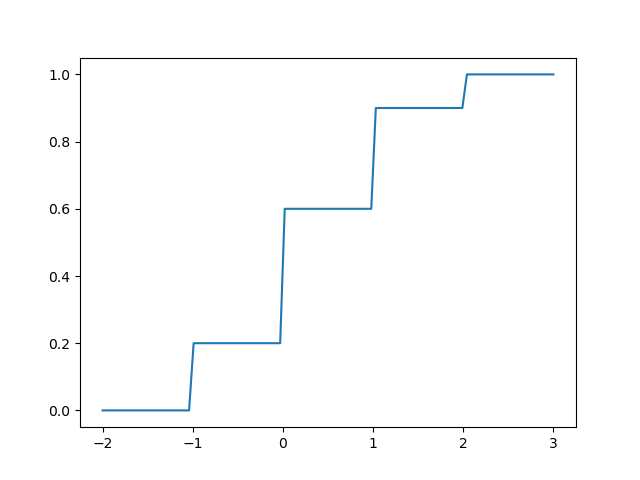
\includegraphics[scale=0.7]{graph_7_1.png}
\end{center}

\begin{task}
\-
\begin{center}
\begin{tabular}{l|rrrrr}
\(\xi\) & -2 & -1 & 0 & 1 & 3\\
\hline
\(p\) & 0.4 & 0.2 & 0.1 &  & 0.2\\
\end{tabular}
\end{center}
\end{task}
\begin{solution}
\[ \sum p_i = 1 \Rightarrow p_4 = 1 - (0.4 + 0.2 + 0.1 + 0.2) = 0.1 \]
\[ E\xi = \sum x_i p_i = -0.3 \]
\[ D\xi = \sum x_i^2p_i - (E\xi)^2 = 3.61 \]
\[ p(-1 \le \xi < 3) = 0.2 + 0.1 + 0.1  = 0.4 \]
\[ F(x) = \begin{cases}
0 & x \le -2 \\
0.4 & -2 < x \le -1 \\
0.6 & -1 < x \le 0 \\
0.7 & 0 < x \le 1 \\
0.8 & 1 < x \le 3 \\
1 & 3 < x
\end{cases} \]
\end{solution}
\begin{task}
В урне два белых и три черных шара. Вынули три шара. Случайная величина \(\xi\) --- число белых среди вынутых. Составить закон распреления, найти числовые характеристики, построить функцию распределения.
\end{task}
\begin{solution}
\-
\begin{center}
\begin{tabular}{l|rrrr}
\(\xi\) & 0 & 1 & 2 & \(\sum\)\\
\hline
\(p\) & 0.1 & 0.6 & 0.3 & 1\\
\end{tabular}
\end{center}
\[ p(\xi = 0) = \frac{\binom{3}{3}}{\binom{5}{3}} = \frac{1}{10} = 0.1 \]
\[ p(\xi = 1) = \frac{\binom{2}{1}\cdot\binom{3}{2}}{\binom{5}{3}} = \frac{2\cdot 3}{10} = 0.6 \]
\[ p(\xi = 2) = \frac{\binom{2}{2}\cdot\binom{2}{1}}{\binom{5}{3}} = \frac{1\cdot 3}{10} = 0.3 \]
\[ E\xi = 0 \cdot 0 + 1 \cdot 0.6 + 2\cdot 0.3 = 1.2 \]
\[ D\xi = 0.6\cdot 1.2 - 1.2^2 = 0.36 \]
\[ \sigma = 0.6 \]
\end{solution}
\begin{task}
Вероятность попадания стрелка \(0.6\). Стрелок сделал 4 выстрела. Случайная величина --- число попаданий
\end{task}
\begin{solution}
\-
\begin{center}
\begin{tabular}{l|rrrrrr}
\(\xi\) & 0 & 1 & 2 & 3 & 4 & \(\sum\)\\
\hline
\(p\) & 0.0256 & 0.1536 & 0.3456 & 0.3456 & 0.1296 & 1\\
\end{tabular}
\end{center}
\[ p(\xi = 0) = 0.4^4 \]
\[ p(\xi = 1) = \binom{4}{3} \cdot 0.6 \cdot 0.4^3 \]
\[ p(\xi = 2) = \binom{4}{2} \cdot 0.6^2 \cdot 0.4^2 \]
\[ p(\xi = 3) = \binom{4}{1} \cdot 0.6^3 \cdot 0.4 \]
\[ p(\xi = 4) = 0.6^4 \]
\[ E\xi = \sum x_i p_i = 2.4 \]
\[ D\xi = \sum x_i^2 p_i - 2.4^2 = 0.96 \]
Это биноминальное распределение поэтому можно применить формулы:
\[ E\xi = np = 4 \cdot 0.6 = 2.4 \]
\[ D\xi = npq = 2.4 \cdot 0.4 = 0.96 \]
\end{solution}
\section{ДЗ}
\label{sec:org33b5fcc}
\begin{task}
В урне 1 белый и 1 черный шар. Два игрока по очереди тянут один шар. Если шар оказался белым, то игра заканчивается, этот игрок побеждает и получает от проигравшего 1 биткоин. Если нет, то в урну возвращается уже 2 черных шара. \\
Случайная величина \(\xi\) --- выигрыш первого игрока. Составить закон распределения, сделать проверку, найти \(E\xi\) и \(D\xi\). Сколько должен дать первый игрок второму игроку за право первого хода, чтобы игра было справедливой?
\end{task}

\begin{task}
Игрок играет в орлянку(с монетой че то) по схеме с удвоением. Если он проигрывает, то удваивает предыдущую ставку. Играет до тех пор пока не выиграет. Случаная величина \(\xi\) --- выигрышь игрока по данной схеме. Найти мат. ожидание и дисперсию.
\begin{enumerate}
\item Бесконечное количество попыток
\item \(N\) попыток
\end{enumerate}
\end{task}
\end{document}
